\chapter{Monte Carlo simulation}

\begin{overview}
  Monte Carlo simulation entails running a deterministic simulation many times with variables chosen from the correct distributions.
  For valid results, the random numbers must be generated correctly, the simulation run correctly and the results collected with correct calculation of the output distributions.
  This chapter explores these aspects of Monte Carlo simulation.
\end{overview}

\section{Introduction}
Monte Carlo simulation is the brute-force algorithm of the statistical world:
\citet{hammersley.handscomb1965monte} compare Monte Carlo simulation to experimental mathematics.
At the heart of the method is the idea that it is often much easier to develop a high-fidelity deterministic model of a process than characterising a stochastic process.
Using these deterministic models, one can estimate the distribution of output variables using input variables generated to conform to a known input distribution.
For this process to work, we need realistic inputs, a good deterministic model and a reliable way of interpreting the results.

% FIXME: We need a nice figure here illustrating the concept and a better
% reference than moody

\citet{sawilowsky2003you} lists the characteristics of a high quality Monte Carlo simulation as follows:
\begin{itemize}
\item the pseudo-random number generator has certain characteristics (e.g. a long “period” before repeating values)
\item the pseudo-random number generator produces values that pass tests for randomness
\item the number of repetitions of the experiment is sufficiently large to ensure accuracy of results
\item the proper sampling technique is used
\item the algorithm used is valid for what is being modeled
\item the study simulates the phenomenon in question.
\end{itemize}

\section{Input generation}
Within the context of MC simulation, ``inputs'' are sources of variance.
Variance can be characterised as ``real'' variance, or external variance and uncertainty, which is inherent in the model, but does not exist in the real process\footnote{We assume here that deterministic models are able to capture the
process behaviour}.
In a sense, the variability of the inputs captures our uncertainty about their behaviour.
We therefore distinguish between varibles that remain fixed during a simulation, but could assume different values for any given simulation, and those that would be expected to assume many values over a given simulation time.
In the first case we simply have to generate values conforming to a known distribution.
In the second, we need to generate realistic input sequences, typically including realistic transitions between the different values they attain.

% FIXME: Create a figure showing the taxonamy of variables.

\section{Pseudo-random number generation}
% TODO: Heavily rewrite with reference to Saucier's ``Computer Generation of Statistical Distributions''
% ~/Downloads/Documents/random_number_generation/random.pdf

% TODO: Flesh out this description
Also see \citet[183]{giordano.fox.ea2009first} for a discussion on random number generation.

As modern computers are deterministic devices, it is theoretically impossible to use them to generate a sequence of truly random numbers~\citep{neumann1951various}.
However, it is possible to generate a (periodic) sequence of numbers that are not significantly different from a random number sequence.
Such a sequence is termed pseudo-random.

% TODO: Find a good reference for George Marsaglia
% http://en.wikipedia.org/wiki/Diehard_tests
% http://en.wikipedia.org/wiki/George_Marsaglia
% http://www.phy.duke.edu/~rgb/General/dieharder.php

\subsection{Uniformly distributed}
The most commonly used distribution for RNGs is the uniform distribution.
Numbers are usually generated in the range of $[0, N)$ where $N$ is some large number.
Continuously distributed values in the range $[0,1)$ are generated from the discrete variable by dividing by $N$.

\subsubsection{Linear congruential generators}
The most popular generators are the linear congruential generators, which take the form \citep[10]{knuth1997art}
\begin{equation}
X_{i+1} = (aX_i +c) (\mod N)
\end{equation}

% TODO: Refer to the use of the Mersenne Twister algorithm
%\begin{quote}
The 1997 invention of the Mersenne twister algorithm, by Makoto Matsumoto and Takuji Nishimura, avoids many of the problems with earlier generators.
It has the colossal period of 219937−1 iterations ($>43\times106,000$), is proven to be equidistributed in (up to) 623 dimensions (for 32-bit values), and runs faster than other statistically reasonable generators.
It is now increasingly becoming the random number generator of choice for statistical simulations and generative modeling.
SFMT, SIMD-oriented Fast Mersenne Twister, a variant of Mersenne twister, is faster even if it's not compiled with SIMD support.
%\end{quote}

Marsaglia suggests the use of XOR-based generators for normal
applications where efficiency is important \citehere.

\subsection{Normally distributed}
Several routines exist to generate normally distributed pseudo-random values.
Most of them involve drawing a number of uniformly distributed values and manipulating them, but some purpose-built algorithms exist~\citehere.

\subsection{Arbitrary distributions}

\subsubsection{Given a CDF}
If the CDF is invertable, it is a simple matter to generate the distribution if one has access to a uniformly random number.
Simply choose this number and calculate the inverse, as shown in figure~\ref{fig:random_inverse}.

\begin{figure}[htbp]
  \centering
  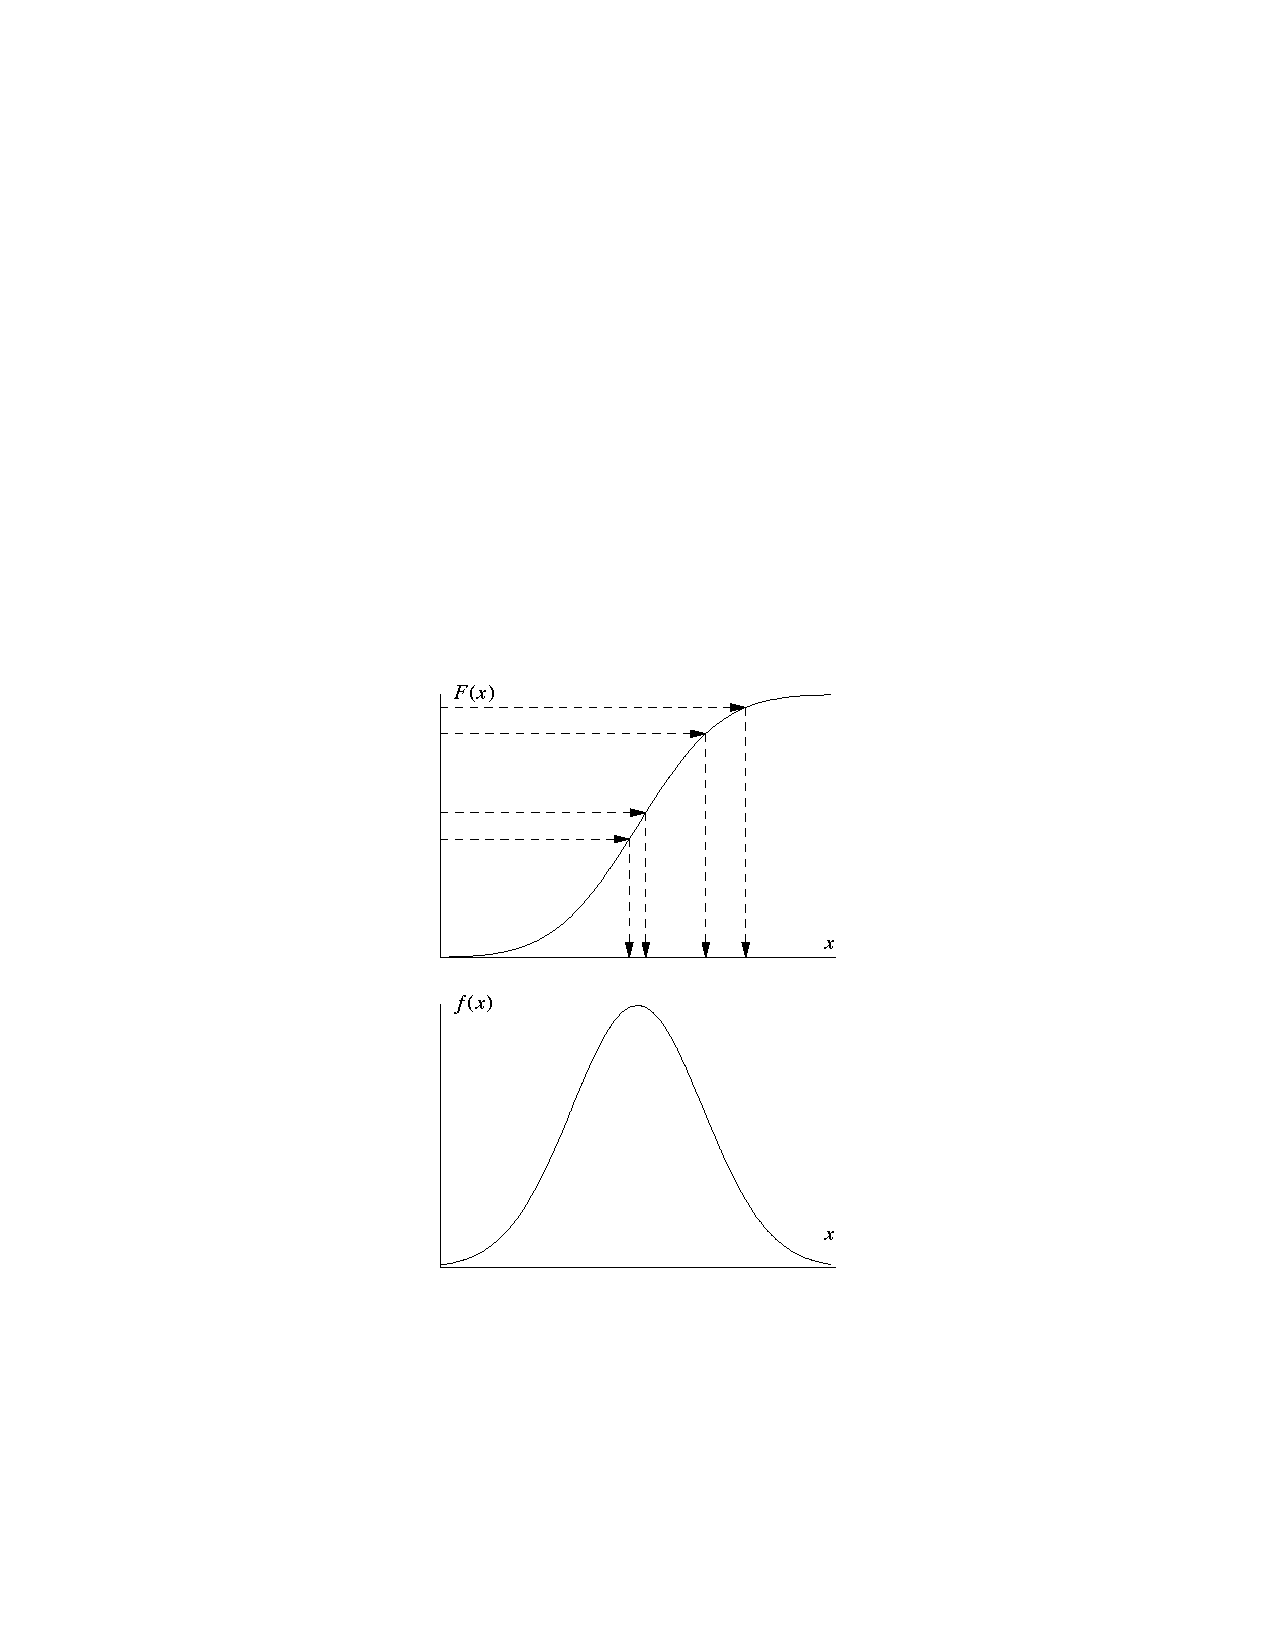
\includegraphics[width=0.5\textwidth]{random_inverse}
  \caption[Generating an arbitrary distribution via the inverse of the CDF]{Generating an arbitrary distribution via the inverse of the CDF \citep{saucier2000computer}}
  \label{fig:random_inverse}
\end{figure}

Therefore, to generate a number distributed with distribution $f(x)$ and invertible cumulative distribution $F(x)$, simply return $F^{-1}(U(0, 1))$.

If the inverse does not exist or is difficult to calculate, it may be necessary to use an acceptance rejection technique.
Such techniques are based on the observation that the probability of generating a point which falls under $f(x)$ is distributed similarly to $f(x)$.
The procedure is to generate two uniform random numbers $X \leftarrow U(x_{\min}, x_{\max})$ and $Y \leftarrow U(y_{\min}, y_{\max})$ then to return $X$ if $X<F(Y)$.

\subsubsection{From data}


\section{Sequence generation}
\subsection{Sequence probabilities}

\section{Introduction}
A simulation is a reproduction under controlled circumstances of a real-life situation.
The term has recently become strongly associated with numeric evaluation of a computer model due to the increase in speed and availability of computing resources.
This increase in speed has led to much interest in stochastic simulation, where processes with elements that are random are simulated.
An attractive branch of stochastic simulation termed Monte Carlo simulation uses deterministic models driven by stochastic input sequences to approximate the distributions of output variables over time.
To do this, a good deterministic model of the process is needed in addition to a good method of generating realistic input sequences.

Correct input sequences are a prerequisite for reliable results from stochastic simulation.
To generate them, the modeller must either generate input sequences by hand, develop a model based on intuition or understanding of the process, or use existing data.
Generating input sequences by hand is a tedious and error-prone process and intuition is not a particularly verifiable source of information.
This means that data-driven model development has been gaining favour steadily as data becomes more accessible.

This chapter is covers three aspects of input signal generation:
First, the basic theory of Markov processes and hidden Markov models is reviewed with a view on using them as generating processes for input models.
Second, signal segmentation is introduced.
This is the first step in identifying state transition probabilities for discrete Markov processes.
In this part, novel work done on the identification of state transitions using multi-objective optimisation is introduced and ideas for future research are posed.
Third, the problem of estimating state transition probabilities from the segmented signals is discussed, touching on the issues that modellers should be aware of.

Markov processes have featured strongly in stochastic sequence identification and generation for many years, but some of the related problems are still active research fields.


\section{Simulation}
% TODO: these paragraphs are duplicated in the statistics area
At the heart of any computer-based stochastic simulation is the generation of pseudo-random numbers.
It is customary to have a good source of uniformly distributed random numbers and to derive other distributions from them using either transformation or rejection methods.

Most modern computer programming languages have at least this source of randomness, and some may include sources for normally distributed random values.
Commonly encountered transform methods can generate normally distributed, Poisson and logarithmically distributed vales from uniformly distributed values.~\citep{gamerman.lopes2006markov}

Direct simulation of Markov processes boils down to moving from state to state with the prescribed probabilities.
A simple way to choose values with specific probabilities is to use the cumulative sum of the probability vector associated with the current state.

\section{Conclusions}
Markov processes provide a simple yet powerful method for generating realistic input sequences.
The theory in this chapter should be enough for the interested reader to get started in this fascinating field and should enable simulation of a system with little additional reading required.
The techniques for segmenting input signals and identifying model parameters are applicable to a broad range of fields and includes novel work on the employment of multi-objective optimisation to signal segmentation and estimation.

The most interesting future work suggested by this research is the use of variable-length multi-objective GAs to segment signals.


% Local Variables:
% TeX-master: "thesis"
% End:
